\documentclass[a4paper]{article}
\usepackage{graphicx} % Required for inserting images
\usepackage{kotex}
\usepackage{amsmath}
\usepackage{subfigure}
\usepackage{verbatim}
\usepackage{indentfirst}
\usepackage{hyperref}
\hypersetup{
    colorlinks=true,
    linkcolor=blue,
    filecolor=blue,      
    citecolor=blue,
    urlcolor=blue,
}

\title{Demo Application of Synchronous Mobile Distance Learning System}
\author{Hosung.Kim}

\begin{document}

\maketitle

\section{서론}
COVID-19 팬데믹의 영향으로 온라인 기반 원격 교육의 수요가 급증하면서, 원격 교육의 중요성을 부각시키는 결정적인 계기가 되었다. 팬데믹 이후에도 원격 교육은 공간적 제약 없는 학습 환경에 대한 지속적인 수요를 충족시키며, 위기 상황의 일시적인 대안을 넘어 새로운 교육 패러다임으로 자리매김하였다.

특히, 스마트폰과 태블릿 등의 모바일 디지털 기기의 보급 확대는 동기식 모바일 원격 교육 시스템의 가능성을 열어주었다. 모바일 원격 교육 시스템은 강사와 학생 간의 즉각적인 피드백을 가능하게 하며 실시간 상호작용을 통해 학습 효과를 극대화한다.

이에 본 보고서에서는 동기식 모바일 원격 교육 시스템에 대한 이해를 목적으로 텍스트 기반 채팅, 강사의 음성 및 영상 공유, PDF 기반 강의 자료 주석 기능 등을 포함한 데모 애플리케이션을 설계 및 구현하였다. 제시된 시스템은, 강사가 iPad로 강의를 진행하며, 학생들은 iPad를 이용하여 강사의 음성과 전면 카메라 영상, PDF 강의 자료 및 애노테이션을 실시간으로 보고 들으면서 상호작용을 할 수 있는 형태로 되어 있다.

\section{설계}
\subsection{구조}
본 시스템은 강사측 모바일 클라이언트, 학생측 모바일 클라이언트, 스트리밍 서버, 채팅 서버로 구성된다. 전체 시스템 구성은 그림\ref{fig:fig1}과 같다.
\begin{figure}[htbp]
    \begin{center}
    \includegraphics[width=0.6\textwidth]{강사와 학생간 데이터 흐름.png}
    \caption{강사와 학생간 데이터 흐름}
    \label{fig:fig1}
    \end{center}
\end{figure}
\newpage
\subsubsection{스트리밍}
강사측 모바일 클라이언트는 음성과 영상을 실시간으로 스트리밍 서버에 전송하고, 학생측 모바일 클라이언트는 스트리밍 서버로부터 데이터를 수신한다. 강사측 모바일 클라이언트에서 전송하는 영상은 강사의 iPad 화면에 표시된 PDF자료와 주석을 녹화한 화면과 전면카메라를 하나의 스트림으로 합성하여 송출한다.
\subsubsection{채팅}
강사와 학생의 모바일 클라이언트는 채팅 서버와 각각 연결되며, 서버는 수신한 메세지를 모든 연결된 세션에게 브로드캐스트한다. 이를 통해 텍스트 기반의 양방향 소통이 가능하며, 강의 중 질문이나 피드백을 실시간으로 주고받을 수 있다.
\subsection{아키텍쳐}
클라이언트 애플리케이션은 Clean Architecture와 MVVM (Model - View - ViewModel) 아키텍쳐 패턴을 결합하여 설계되었다. Clean Architecture는 애플리케이션을 계층화하여 각 계층의 책임을 명확하게 함으로써, 재사용성과 테스트 용이성을 높이는 데 목적이 있다. 본 데모 애플리케이션은 Data, Domain, Presentation 세 계층으로 구성된다.
\begin{figure}[htbp]
    \begin{center}
    \includegraphics[width=0.6\textwidth]{아키텍쳐.png}
    \caption{아키텍쳐}
    \label{fig:fig2}
    \end{center}
\end{figure}

Data 계층은 Network, DTO, Repository(Implementation)로 구성되며, 서버와의 직접적인 통신을 담당한다.

Domain 계층은 Entity, Repository(Protocol), UseCase로 구성되며, 핵심 데이터와 비즈니스 로직을 포함한다.

Presentation 계층은 ViewModel, ViewController로 구성되고, UI를 통해 User와 직접 소통한다.

서버와 클라이언트 간의 데이터 흐름은 다음과 같다.
서버로부터 데이터를 수신하는 경우, Network가 서버로부터 DTO 형태의 데이터를 전달받는다. 해당 데이터는 Repository에서 Entity로 변환되고 UseCase를 거쳐 ViewModel에 전달된다. ViewController는 ViewModel의 상태 변화를 관찰하고 있다가 변경사항이 발생하면 이를 UI에 반영한다.
서버로 데이터를 전송하는 경우, ViewController에서 ViewModel, UseCase, Repository를 통해 값을 전달한다. Repository를 거치며 Entity는 DTO형태로 변환되고 최종적으로 Network를 통해 서버로 전송한다.
\newpage
\section{구현}
\begin{figure}[htbp]
    \begin{center}
        \subfigure[테스트]{
            \includegraphics[width=0.8\linewidth]{test.jpeg}
        }
        \subfigure[강사 측 클라이언트의 유저 인터페이스]{
            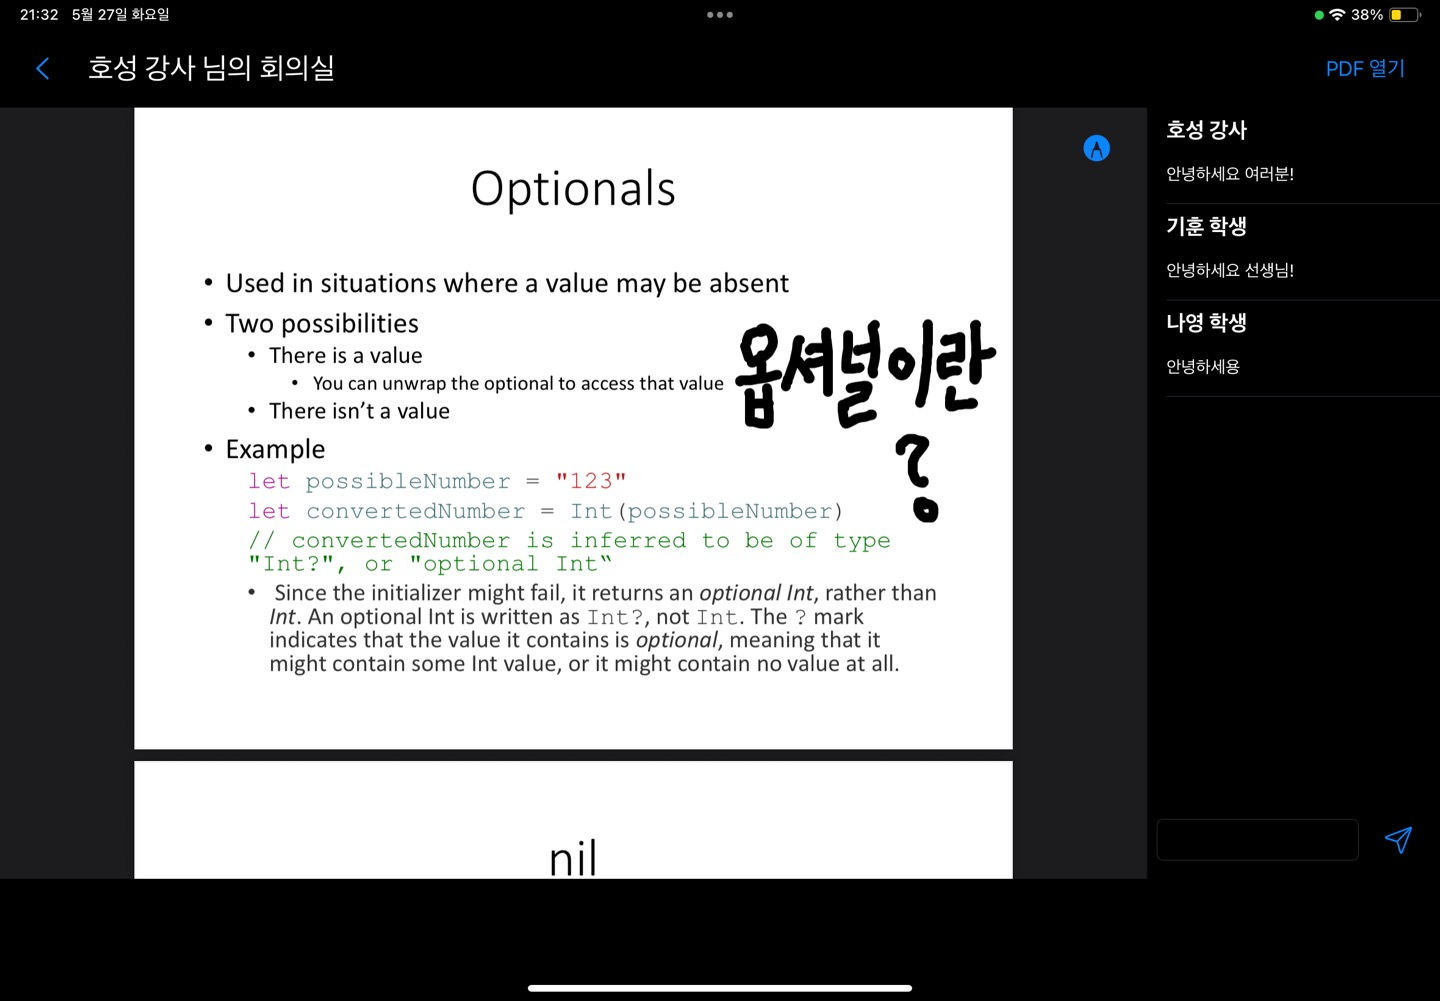
\includegraphics[width=0.4\linewidth]{intructor.jpeg}
        }
        \subfigure[학생 측 클라이언트의 유저 인터페이스]{
            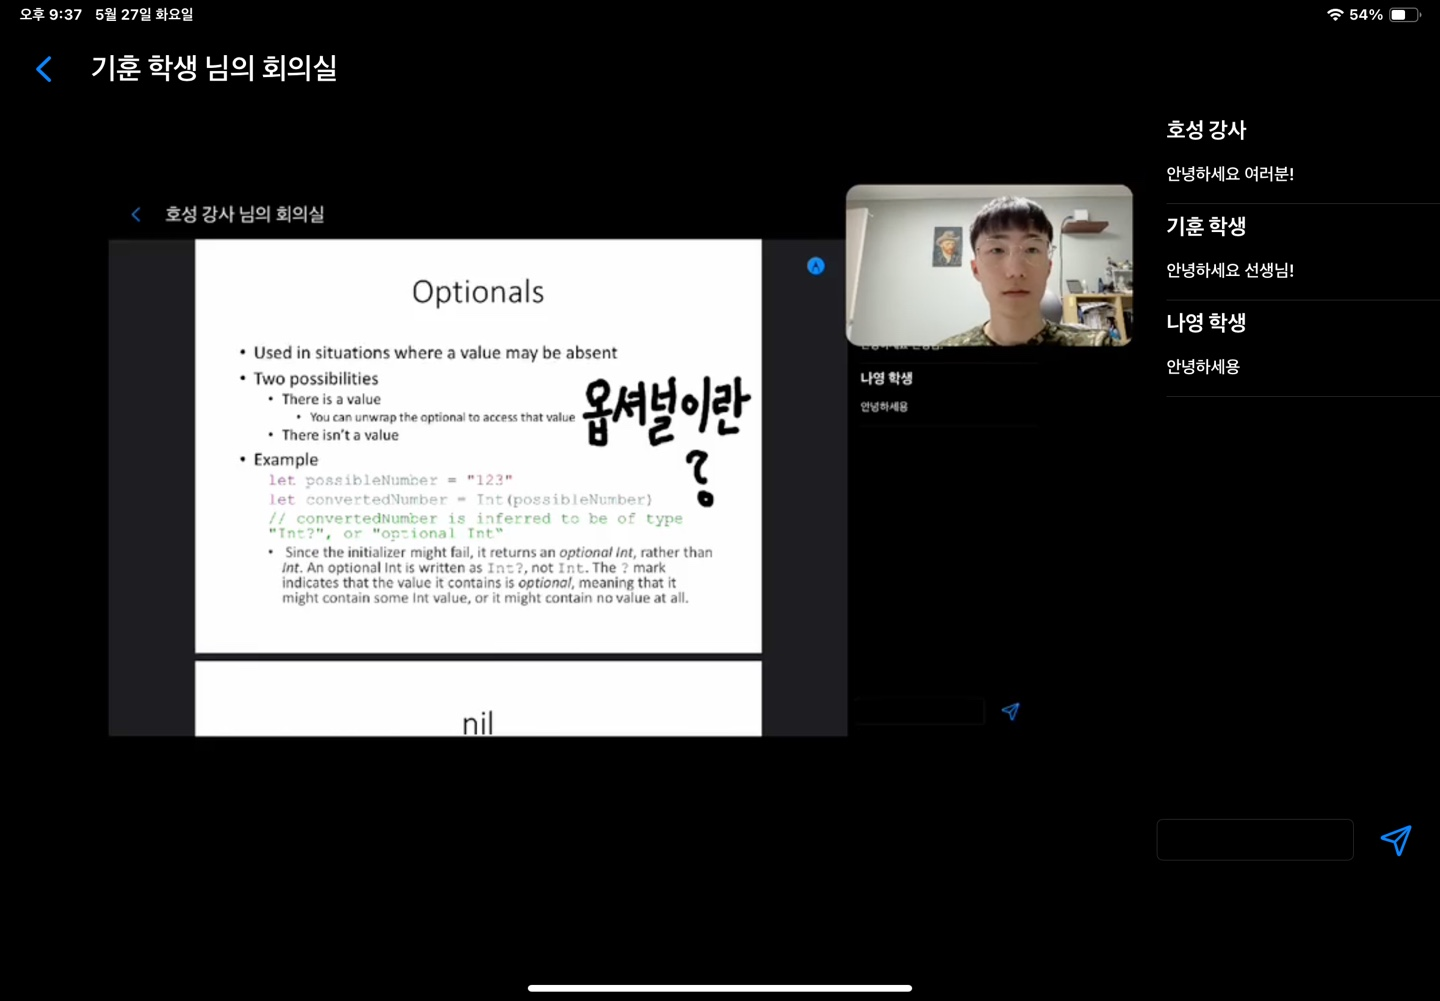
\includegraphics[width=0.4\linewidth]{student.jpeg}
        }
        \caption{구현 모습}
        \label{fig:fig3}
    \end{center}
\end{figure}

\subsection{스트리밍}
스트리밍 기능은 RTMP (Real-Time Messaging Protocol)를 기반으로 구현하였다. 초기 설계 단계에서는 WebRTC 프로토콜의 도입도 고려되었으나, 본 데모 애플리케이션의 구조상 Instructor 클라이언트는 송신 전용, Student 클라이언트는 수신전용의 단방향 흐름을 갖기 때문에, 구현의 단순성과 안정성을 고려하여 RTMP를 최종적으로 채택하였다.

서버는 NGINX기반의 RTMP 스트리밍 서버를 사용하였으며, nginx.conf 설정 파일만 수정함으로써 간단하게 구축할 수 있다.

클라이언트측 구현에는 HaishinKit.swift\cite{HaishinKit} 라이브러리를 활용하였다.
RTMPService 클래스는 해당 라이브러리를 통해 RTMP 서버와의 연결을 설정하고 Instructor 또는 Student의 역할에 따라 수신이나 송신의 역할을 한다.
StreamService에서는 HaishinKit.swift 라이브러리의 MediaMixer를 활용하여 강사의 음성, 강사의 전면 카메라 영상, 화면 녹화 (PDF 및 주석)를 하나의 스트림으로 합성하여 송신한다.
\subsection{채팅}
채팅은 STOMP (Simple Text Oriented Messaging Protocol) 기반의 Websocket 통신으로 구현되었다.
서버는 Spring Boot Starter Web Socket Framework를 사용하여 개발하였다.
클라이언트는 SwiftStomp\cite{SwiftStomp} 라이브러리를 사용하여 개발하였다. SwiftStomp는 STOMP 메세지 전송 및 구독, 핑-퐁 핸들링, 자동 재연결 등의 기능을 지원하므로 안정적인 통신 환경을 제공한다.

WebSocketService는 STOMP 프로토콜에 따라 서버와 연결을 설정하고 메세지 송수신을 담당한다. 서버로부터 메세지를 수신하면 Combine 프레임워크의 PassthroughSubject를 통해 해당 메세지를 방출하고 ViewController에서 이를 구독하고있다가 UI에 반영한다.

\subsection{PDF 및 Annotation}
강의 자료 공유는 PDF 문서를 기반으로 이루어지며 Apple 기본 프레임워크 PDFKit을 활용하여 구현하였다. UIDocumentPickerViewController를 통해 강사가 기기에 저장된 PDF 파일을 선택하면 해당 파일의 링크를 가져와서 PDFView로 화면에 출력된다.

Annotation은 PDFKit의 PDFPageOverlayViewProvider를 사용하여 각 PDFPage에 CanvasView를 overlayView로 추가하여 구현하였다.

CanvasView는 터치 이벤트를 override하여 UIBezierPath로 배열에 저장하는 방식으로 동작한다.

PDF 문서 스크롤과 그리기 기능 간의 충돌을 방지하기 위해, 그리기 모드 토글 버튼을 제공한다. 그리기 모드를 활성화하면 PDFView의 isScrollEnabled를 비활성화하여 터치이벤트에 따라 주석 작성이 가능해지고, 그리기 모드를 비활성화하면 기존의 PDF 탐색 기능을 다시 사용할 수 있다.

강사의 화면은 스트리밍 시, 음성 및 전면 카메라 영상과 함께 송출되며, 이 과정에서 PDFView와 Annotation 역시 함께 전달된다.

\section{결론}
본 보고서에서는 iPadOS 기반의 동기식 모바일 원격 교육 시스템에 대한 이해를 목적으로 데모 애플리케이션을 설계 및 구현하였다.

MacBook M3 Pro에서 스트리밍 서버와 채팅 서버를 구동하고, iPad Air 3대를 활용하여 강사 1인과 학생2인의 환경에서 테스트를 진행한 결과, 1초 이내의 지연으로 실시간 강의 및 상호작용이 원할하게 수행됨을 확인하였다.

다만, 현재까지 개발된 프로토타입 시스템에서는 단일 강의실 환경에서 제한된 인원으로만 테스트된 초기 단계의 시스템으로, 실제 서비스 환경에 적용되기 위해서는 보다 다양한 환경에서의 테스트와 기능 확장이 필요하다. 향후에는 다수의 강의실 생성 기능을 추가하고 M:N 환경에서의 안정성과 성능을 검증할 계획이다.

전체 소스코드는 \href{https://github.com/H0sungKim/CollaborativeComputingLab}{https://github.com/H0sungKim/CollaborativeComputingLab}에서 확인할 수 있다.
\newpage
\begin{thebibliography}{1}
\bibitem{HaishinKit}
HaishinKit.swift. \href{https://github.com/HaishinKit/HaishinKit.swift}{https://github.com/HaishinKit/HaishinKit.swift}
\bibitem{SwiftStomp}
SwiftStomp. \href{https://github.com/Romixery/SwiftStomp}{https://github.com/Romixery/SwiftStomp}
\end{thebibliography}

\end{document}
